\chapter[Including Figures]{Including Figures}
\label{ch:chapter2}


\section{Introduction}

Chapter 1 introduced including equations. In this chapter I will show how figures are included


\section{Figures}

Here is a figure. A useful way to define the width of the figure is by some fraction of the textwidth. Depending on how much white space is around the figure you'll have to play around with this to get it to the size you want it.

\begin{figure}[!hbt]
    \centering
    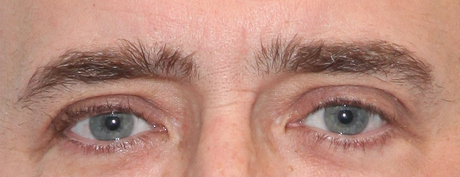
\includegraphics[width=0.8\textwidth]{chapter2_figures/GuessWho.jpg}
    \caption{Can you guess whose eyes these belong to?}
    \label{fig:guess who}
\end{figure}

%\clearpage
\section{Common issues}

Placement of figures is really the only difficulty you'll likely encounter. Often \LaTeX will end up placing the figure too far below where you want it, or even in the next section.

\begin{figure}[!hbt]
    \centering
    
\includegraphics[width=0.9\textwidth]{chapter2_figures/code.png}
    \caption{Not sure that programming would be feasible without copy/paste}
    \label{fig:code}
\end{figure}

In Fig. \ref{fig:code}, the [!hbt] options specified after `begin figure' tell \LaTeX where to try to place the figure in order. First try placing here as specified in the tex file (h), otherwise try at the bottom of the page (b), otherwise try placing at the top of the page (t). The exclamation point specified to overrule any behaviour for figure placement that \LaTeX may have (e.g. from the document class I think?).

Sometimes the figure will end up in the next section, not what we want! As a last resort I will add the clearpage just before the next section forcing placement of figures/tables before the new section starts. You might end up with some extra white space but it's a compromise sometimes we have to make.


\begin{figure}[!hbt]
    \centering
    
\includegraphics[width=\textwidth]{chapter2_figures/yesbutno.png}
    \caption{By the time we come to write up, we've all been asked this at least once. This is the honest answer.}
    \label{fig:yes but no}
\end{figure}

%\clearpage
\section{Next section}

Here's some \textit{Lorem ipsum} to bulk out the text and show that the figure is being placed in this section, despite being part of the previous section. Uncommenting the clearpage command just above the section command will force the figure to be placed, then clear the page before coming to this section.

Fun fact, \textit{Lorem ipsum} is typically a corrupted version of \textit{De finibus bonorum et malorum}, a first-century BC text by the Roman statesman and philosopher Cicero, with words altered, added, and removed to make it nonsensical, improper Latin (according to Wikipedia anyway). It is used as placeholder text since the word length distribution is about the same as English and so serves as a useful representation of what text will end up looking like (in terms of number of words on a line etc).

\lipsum[1-2]